\documentclass{ximera}

\title{Fractions Intro}

\begin{document}
\begin{abstract} We think about what it means to be a fraction. You will need a piece of paper (or two) for this activity. \end{abstract}
\maketitle


\begin{problem}
Take out a sheet of paper. Fold this paper to show what $\frac{1}{5}$ looks like.
\end{problem}


\begin{problem}
What was important about your process in the last problem?
\end{problem}


\begin{problem}
Now, fold your paper to show what $\frac{3}{5}$ looks like.
\end{problem}


\begin{problem}
What was important about your process in the last problem? How does your process compare to your process for the first fraction?
\end{problem}


\begin{problem}
Using what you've learned, come up with a definition for the fraction $\frac{A}{B}$ where $A$ and $B$ are both whole numbers.
\end{problem}

\newpage

Now that we have a definition for fractions, let's practice applying it in various situations. 

\begin{problem}
\begin{itemize}
	\item Draw a picture that shows $\frac{2}{7}$ of a pan of brownies. Explain how you know your answer is correct.
	\item What would $\frac{2}{7}$ look like on a number line? Explain how your process of drawing this fraction is connected to our meaning of fractions.
	\item Draw a picture that shows $\frac{7}{2}$ of a pan of brownies. Explain how you know your answer is correct.
	\item What would $\frac{7}{2}$ look like on a number line? Explain how your work is connected to the meaning of fractions. 
	\item What does our work in this problem tell us about why our definition of fractions is {\bf not} ``$A$ parts out of $B$''?
\end{itemize}
\end{problem}

\begin{problem}
	The rectangle below is $\frac{3}{8}$ of some other rectangle. Draw the other rectangle. Explain how your thinking is connected to our definition of fractions. 
	
	\begin{image}
		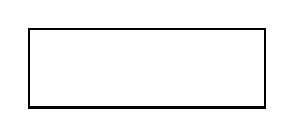
\begin{tikzpicture}
			\draw[thick] (0,0) rectangle (3,1);
		\end{tikzpicture}
	\end{image}
\end{problem}





\newpage
\begin{instructorNotes}


{\bf Main Goal:} We use students' ideas and language to develop the definition of a fraction given in the textbook. 


{\bf Overall Picture:} 
We want to define the fraction $\frac{A}{B}$ in the following way. First, we identify a whole object associated with the fraction. We cut the fraction into $B$ equal-sized pieces, each of which is $\frac{1}{B}$ of the whole. Then, we select or make $A$ copies of one of those pieces, or $A$ copies of $\frac{1}{B}$. Check the textbook for the wording there as well!

\begin{itemize}
	\item An important note here: these fractions are missing the associated whole. At the end of the activity (if no one has brought it up previously), you'll want to make a big deal about this because we don't want students to make this same ``mistake''.
	\item The first fraction focuses on the meaning of the denominator, since the numerator is $1$. We hope that students notice that we need to cut our whole into five equal pieces. Their folding is probably not accurate, which is okay. Students may bring up this inaccuracy.
	\item The second fraction focuses on the meaning of the numerator, since we are using the same denominator. The students should select three copies of what they had in the first fraction, but they will probably not see this without being prompted to think about how these two fractions are connected.
	\item Once the students have brought forth their ideas, wrap up the discussion by presenting the book's definition. Highlight how each piece was brought up by the students!
	\item You might also help students notice that some students might have held their paper in the reverse direction, thus showing their ``one fifth'' in a different shape or area.  Similarly, folding a half sheet of paper yields a ``smaller'' image of $\frac15$.  We want to call their attention to the fact that what makes the image $\frac15$ is its relationship to the whole, not its size, shape, or area.
	\item In Problem 6, we draw fractions using rectangles and number lines. Students have the opportunity to practice with the meaning of fractions and their first experience with thinking about fractions larger than one. Have students present their work, and if you can keep all of the pictures up at the same time then it will be helpful to ask students to compare and contrast the first four parts. Wrap up by using this work to talk about why ``$A$ out of $B$'' doesn't make sense for number lines or for improper fractions, since the ``out of'' may not be the whole. 
	\item Many students struggle with improper fractions, so drawing $\frac{7}{2}$ may be a challenge.
	\item Number lines can present a challenge in determining what the whole should be. We want to take the whole to be the unit length, or the distance between $0$ and $1$. Watch out for students drawing whole numbers $1$ through $7$ and marking the tick at $2$.
	\item On the last problem, the type of thinking where we represent the amount we have in terms of the numerator is more difficult for students than when the box represents our whole, but is very useful for our students as we move forward. For instance, it's natural to cut the yellow box into eight equal pieces, and shade three of those pieces (three copies of $\frac18$). However, we want to think of the   box as the three pieces we have, and add the rest of the pieces on.
\end{itemize}



{\bf Good Language:} Students often like to say things like $\frac{3}{5}$ means ``3 out of 5''. This language is okay for some fractions, but problematic for others. (What does ``12 out of 4'' mean?) If you are hearing this language during discussion, you might bring up the fact that our actual definition of fractions is different than this. We'll focus on this in problem 6.

You will want to introduce the terminology of ``numerator'' and ``denominator'' as appropriate during this discussion. Some students will have forgotten!

It's also important to begin emphasizing the order in which we work with a fraction. First, we identify the whole. Then, we deal with the denominator, and finally we deal with the numerator. 



{\bf Suggested Timing:} The first page should be done in whole-class discussion, and should take roughly 15 minutes. After that, for the second page give students about 5-8 minutes to work on the problems, then have students present and discuss with the rest of the time.

\end{instructorNotes}





\end{document}